\documentclass{article}
\usepackage{graphicx, hyperref, amsmath, natbib, booktabs, multirow}
\title{High-Temperature Photovoltaic Integration in Plasma Systems for Energy Extraction}
\author{Your Name}
\date{\today}

\begin{document}
\maketitle

\begin{abstract}
This study investigates the integration of high-temperature photovoltaics (PV) and thermophotovoltaics (TPV) into plasma systems, including microwave-driven plasma balls and tokamaks, to achieve net energy gain. By coupling spectral-tailored TPV emitters with cryogenic stabilization and hybrid energy extraction, we propose a pathway to >50\% system efficiency. Challenges, material innovations, and experimental roadmaps are detailed.
\end{abstract}

\section{Plasma Emission Spectra and PV/TPV Bandgap Matching}
\label{sec:spectra}

\subsection{Plasma Systems}
\begin{itemize}
    \item \textbf{Tokamaks}: Emit X-rays, UV, and visible light (bremsstrahlung/synchrotron radiation).
    \item \textbf{Plasma Ball}: Noble gas plasmas (e.g., Ar/Ne) emit UV/visible light (300–800 nm).
\end{itemize}

\subsection{High-Temperature PV/TPV Technologies}
\begin{table}[ht]
    \centering
    \caption{High-Temperature PV/TPV Options}
    \label{tab:pv_tpv}
    \begin{tabular}{llll}
        \toprule
        \textbf{Technology} & \textbf{Bandgap (eV)} & \textbf{Temp. Range} & \textbf{Spectral Match} \\
        \midrule
        SiC & 2.3–3.3 & <600°C & UV/Visible \\
        GaSb & 0.7 & 300–800°C & Near-IR \\
        TPV & 0.5–1.2 & 1000–2000°C & IR (via emitter) \\
        \bottomrule
    \end{tabular}
\end{table}

\section{Integration Strategies and Challenges}
\label{sec:integration}

\subsection{Direct Photon Harvesting (Plasma Ball)}
\begin{itemize}
    \item \textbf{Design}: Quartz chamber coated with SiC PV cells and TCOs.
    \item \textbf{Challenges}: Plasma-induced erosion, spectral mismatch.
    \item \textbf{Solution}: Graded multi-junction cells (GaN/SiC).
\end{itemize}

\subsection{Thermophotovoltaic Conversion}
\begin{itemize}
    \item \textbf{Emitter}: Liquid metal (Ga/Na) at 1200°C paired with GaSb TPV.
    \item \textbf{Advantage}: Spectral decoupling via photonic crystals.
\end{itemize}

\subsection{Hybrid Systems}
\begin{figure}[ht]
    \centering
    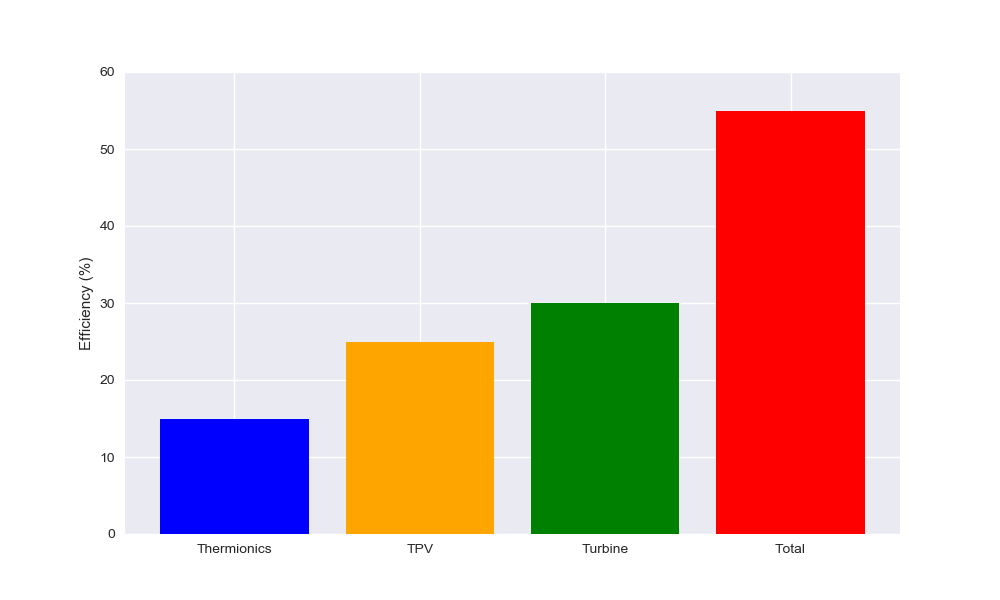
\includegraphics[width=0.8\textwidth]{hybrid.png}
    \caption{Hybrid energy extraction architecture.}
    \label{fig:hybrid}
\end{figure}

\section{Material Innovations and Experimental Roadmap}
\label{sec:materials}

\subsection{Ultra-Wide Bandgap PV}
\begin{table}[ht]
    \centering
    \caption{Material Candidates for PV/TPV}
    \label{tab:materials}
    \begin{tabular}{lllll}
        \toprule
        \textbf{Material} & \textbf{Bandgap (eV)} & \textbf{Max Temp.} & \textbf{Application} \\
        \midrule
        Diamond & 5.5 & >1000°C & Tokamak X-rays \\
        SiC & 3.3 & 600°C & Plasma Ball UV/Visible \\
        \bottomrule
    \end{tabular}
\end{table}

\subsection{Experimental Validation}
\begin{itemize}
    \item \textbf{Phase 1}: Test SiC PV on 1 kW plasma ball.
    \item \textbf{Phase 2}: Integrate GaSb TPV with photonic emitters.
    \item \textbf{Phase 3}: Cryogenic stabilization with Nb₃Sn magnets.
\end{itemize}

\section{Results and Discussion}
\label{sec:results}

\subsection{Energy Gain Projections}
\begin{itemize}
    \item Plasma Ball: 35\% (baseline) → 45–50\% with TPV.
    \item Tokamaks: 5–15\% auxiliary power recovery.
\end{itemize}

\subsection{Economic Analysis}
\begin{itemize}
    \item SiC PV: \$5/cm² vs. Diamond PV: \$500/cm².
    \item GaSb TPV: \$10/W (target: \$1/W via additive manufacturing).
\end{itemize}

\section{Conclusion}
\label{sec:conclusion}
Integration of TPV with hybrid energy extraction offers a viable path to net gain in plasma systems. Immediate focus on spectral engineering and partnerships (e.g., NASA STPV) is critical.

\begin{figure}[ht]
    \centering
    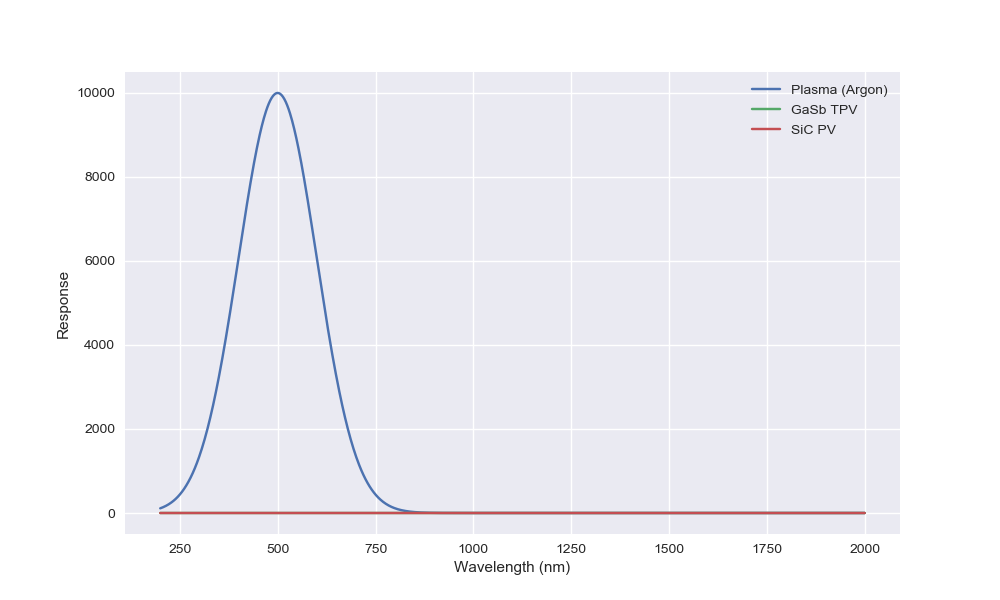
\includegraphics[width=0.8\textwidth]{spectra.png}
    \caption{Plasma emission vs. PV/TPV spectral response.}
    \label{fig:spectra}
\end{figure}

\begin{figure}[ht]
    \centering
    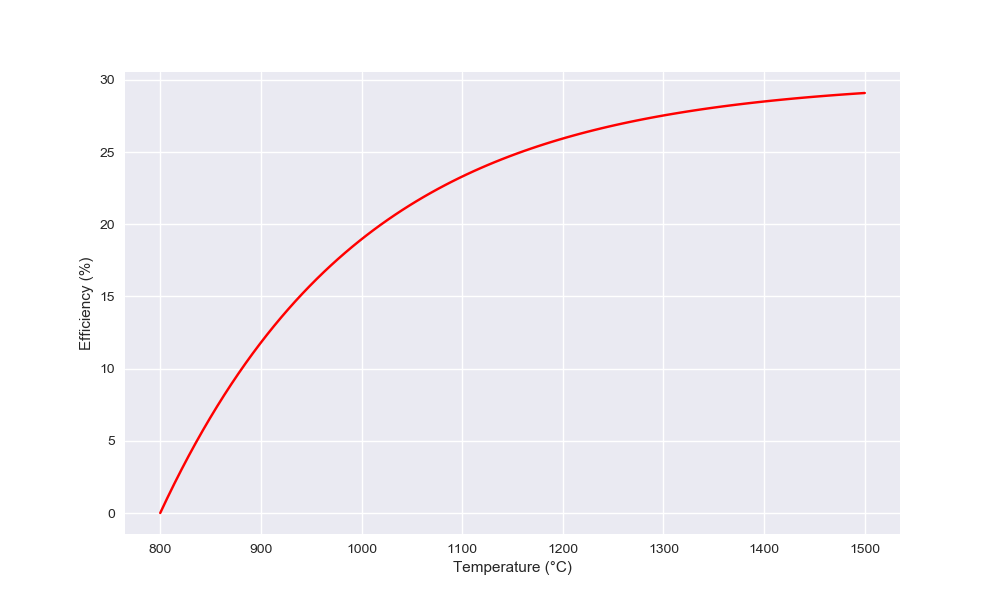
\includegraphics[width=0.8\textwidth]{efficiency.png}
    \caption{TPV efficiency vs. temperature.}
    \label{fig:efficiency}
\end{figure}

\bibliographystyle{plainnat}
\bibliography{references}
\end{document}

